\documentclass[a4paper]{article}

\usepackage[cm]{fullpage}
\usepackage{parskip}
\usepackage{graphicx}
\usepackage{subfig}

\renewcommand{\familydefault}{\sfdefault}

\usepackage{hyperref}
\hypersetup
{
    colorlinks,
    citecolor=blue,
    filecolor=blue,
    linkcolor=black,
    urlcolor=blue
}

\title{Semantic Audio Feature Extraction (SAFE) Plug-Ins}
\author{}
\date{}

\begin{document}

\maketitle

\section*{Introduction}
	Hi there, thanks for downloading the SAFE plug-ins.

	These plug-ins are part of a research project being undertaken by two research groups:

	\begin{itemize}
		\item \href{http://www.bcu.ac.uk/tee/dmt/research}{The Digital Media Technology group at Birmingham City University.}

		\item \href{http://c4dm.eecs.qmul.ac.uk/}{The Centre for Digital Music at Queen Mary University of London.}
	\end{itemize}

	\subsection*{Audio Semantics}
		During your adventures in music production you will have most likely used words like bright, flabby or fuzzy to describe a sound. Our brains are pretty good at choosing these words. Take Mr. Obama here for example:

		\begin{figure}[h!]
			\centering
			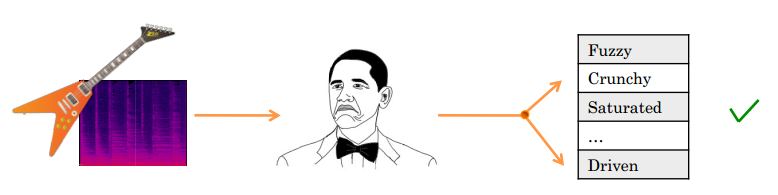
\includegraphics[width=0.8\textwidth]{Images/Obama.png}
		\end{figure}

		He listens to the wicked guitar lick and comes up with some words to describe its timbre. He can then use these words to describe the sound to other people. He might say during his next speech ``You know what. I really like a good fuzzy guitar tone''. Most people listening would then be able to formulate some kind of idea about how he likes his guitars to sound.

		This mastery of language allows us to communicate with others about how we think things should sound. But what if Mr. Obama wants to make his guitar sound fuzzy but he doesn't know how? If only he could give his recorded guitar track to a computer and say ``Make it sound fuzzy''. The trouble is computers are not very good at `hearing' the timbre of a sound.

		\begin{figure}[h!]
			\centering
			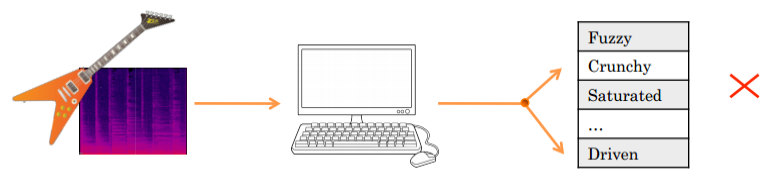
\includegraphics[width=0.8\textwidth]{Images/Computer.png}
		\end{figure}

		A person (such as yourself) might take Mr. Obama's guitar track and apply a distortion plug-in, tweaking the parameters to achieve that holy grail of fuzziness. A computer though, does not know what fuzzy sound like so how does it know what parameters to tweak.

		Here is where the SAFE project steps in. Our goal is to try and define just what words like fuzzy mean so the computer can set the parameters of a plug-in for us. In order to do this successfully we need to collect data about what sort of words people use and what properties of an audio signal they are using them to describe.

		That's where you come in.

	\subsection*{SAFE Plug-Ins}
		The SAFE plug-ins are a series of audio plug-ins which allow the user to provide timbral descriptions of the audio they are processing with them. The plug-in then analyses the audio and saves the data to our server. This data is collected from all the users and analysed to give a general synopsis of what types of sound a given descriptor is used for. 

		All this information can then be used to create a series of `semantic plug-in settings'. Users will be able to load plug-in settings by typing in descriptive words of how they want the audio to sound.

		The more people who upload descriptors to the server the better the downloaded plug-in settings will get.

\section*{Plug-In Use}
	The plug-ins work just like any other audio plug-ins you might use. Just load them up in your DAW of choice (sorry no ProTools at the moment) and your ready to go.

	Here is the interface for the EQ plug-in:

	\begin{figure}[h!]
		\centering
		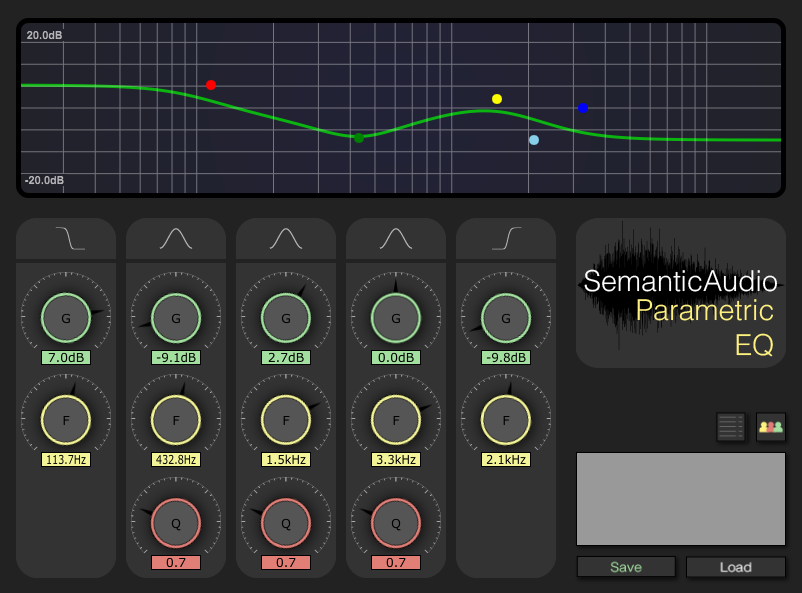
\includegraphics[width=0.9\textwidth]{Images/EQ.png}
	\end{figure}
	
	It works just like any other EQ out there, the bit of interest is the group of buttons in the bottom right corner. These allow you to save and load `semantic plug-in settings.
	
	\newpage
	\subsection*{Saving Plug-In Settings}
		Once you have used one of our plug-ins to get your audio sounding how you want it you can save the plug-in setting.

		This is just a simple task of writing some descriptors in the text box and hitting save.

		\begin{figure}[h!]
			\centering
			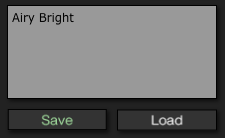
\includegraphics[scale=1]{Images/Saving.png}
		\end{figure}

		As part of the saving process the plug-in has to analyse the audio you are working on. In order to do this the audio needs to be playing when you hit save. Once you hit save the save button will notify you that the plug-in is recording the features of your audio. During this time you should not change any of the plug-in parameters. If you do the plug-in will tell you off and cancel the saving process.

		The plug-in can be set to save either locally on your own machine or to our server. This is done using the save location button which looks like this:

		\begin{figure}[h!]
			\centering
			\subfloat[Save Locally]
			{
				\makebox[0.3\textwidth]{
\includegraphics[scale=1]{Images/usr_local.png}}
			}
			\subfloat[Save to Server]
			{
				\makebox[0.3\textwidth]{
\includegraphics[scale=1]{Images/usr_global.png}}
			}
		\end{figure}

		The currently visible image will determine where the data is saved to. Clicking on the button will toggle the mode. The mode will default to saving to the server if the plug-in is able to access the internet. If not it will save locally.

		To aid in the analysis of the data there is also an option to enter additional information about the audio you are working on and yourself. You can do this by clicking the additional information button which looks like this:

		\begin{figure}[h!]
			\centering
			
\includegraphics[scale=1]{Images/metadata.png}
		\end{figure}

		This will present you with a data entry screen that looks like this:

		\begin{figure}[h!]
			\centering
			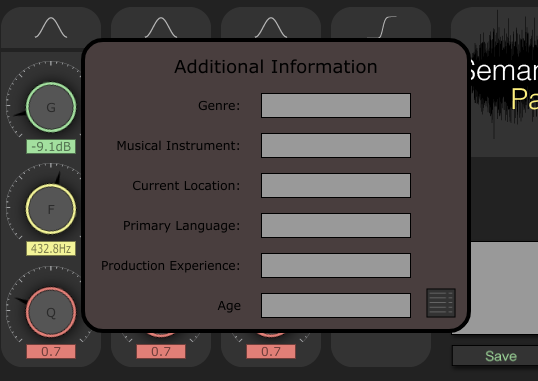
\includegraphics[width=0.6\textwidth]{Images/MetaDataScreen.png}
		\end{figure}

		This information will be used to help in creating genre/instrument specific plug-in settings.

	\subsection*{Loading Plug-In Settings}
		On pressing the load button you will be presented with the following screen:

		\begin{figure}[h!]
			\centering
			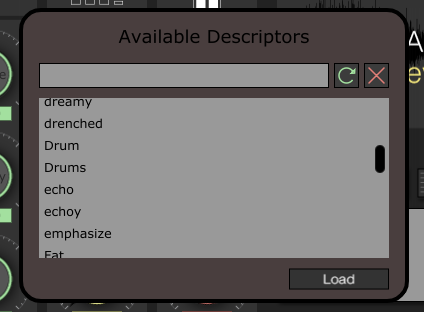
\includegraphics[width=0.6\textwidth]{Images/Loading.png}
		\end{figure}

		This present a list of the current descriptors available to load. The list can be searched using the query box at the top of the screen.

\newpage
\section*{Reaper Problems}
	If you are using Reaper you may need to do some additional setup to get the plug-ins working properly. When adding plug-ins to a channel, right click on the plug-in name and select ``Send all keyboard input to plug-in''. 

	\begin{figure}[h!]
		\centering
		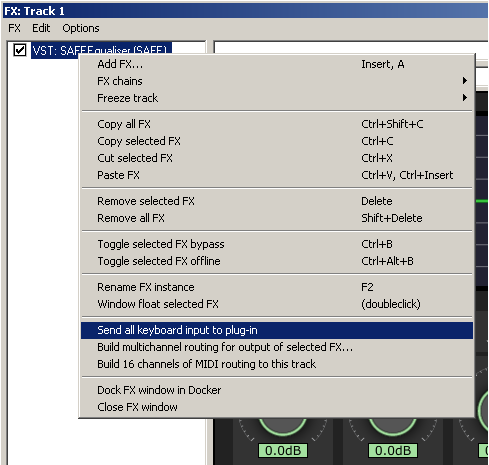
\includegraphics[scale=1]{Images/Reaper.png}
	\end{figure}

\section*{Have A Nice Day Now!}
	Enjoy using these plug-ins and please try not to write too many swear words in the descriptor box.
\end{document}
